
\documentclass[11pt,a4paper,oneside]{book}
\usepackage{a4wide}                     % Iets meer tekst op een bladzijde
\usepackage[dutch]{babel}               % Voor nederlandstalige hyphenatie (woordsplitsing)
\usepackage{amsmath}                    % Uitgebreide wiskundige mogelijkheden
\usepackage{amssymb}                    % Voor speciale symbolen zoals de verzameling Z, R...
\usepackage{makeidx}                    % Om een index te maken
\usepackage{url}                        % Om url's te verwerken
\usepackage{graphicx}                   % Om figuren te kunnen verwerken
\usepackage[small,bf,hang]{caption}     % Om de captions wat te verbeteren
\usepackage{xspace}                     % Magische spaties na een commando
\usepackage[latin1]{inputenc}           % Om niet ascii karakters rechtstreeks te kunnen typen
\usepackage{float}                      % Om nieuwe float environments aan te maken. Ook optie H!
\usepackage{flafter}                    % Opdat floats niet zouden voorsteken
\usepackage{listings}                   % Voor het weergeven van letterlijke text en codelistings
\usepackage[round]{natbib}              % Voor auteur-jaar citaties.
\usepackage[nottoc]{tocbibind}			% Bibliografie en inhoudsopgave in ToC; zie tocbibind.dvi
\usepackage{eurosym}                    % om het euro symbool te krijgen
\usepackage{textcomp}                   % Voor onder andere graden celsius
\usepackage{fancyhdr}                   % Voor fancy headers en footers
\usepackage[Gray,squaren,thinqspace,thinspace]{SIunits} % Om elegant eenheden te zetten
\usepackage[version=3]{mhchem}          % Voor elegante scheikundige formules
\usepackage{subcaption}
% Volgend package is niet echt nodig. Het laat echter toe om gemakkelijk elektronisch
% te navigeren in je pdf-document. Deze package moet altijd als laatste ingeladen worden.
\usepackage[a4paper,plainpages=false]{hyperref}    % Om hyperlinks te hebben in het pdfdocument.


%%%%%%%%%%%%%%%%%%%%%%%%%%%%%%
% Algemene instellingen van het document.
%%%%%%%%%%%%%%%%%%%%%%%%%%%%%%

% De splitsingsuitzonderingen
\hyphenation{back-slash split-sings-uit-zon-de-ring}

% Het bibliografisch opmaak bestand.
% ZORG ERVOOR DAT bibliodutch.bst ZICH IN JE WERKDIRECTORY BEVINDT!!!
\bibliographystyle{bibliodutch}

\setlength{\parindent}{0cm}             % Inspringen van eerste lijn van paragrafen is niet gewenst.

\renewcommand{\baselinestretch}{1.2} 	% De interlinie afstand wat vergroten.

\graphicspath{{figuren/}}               % De plaars waar latex zijn figuren gaat halen.

\makeindex                              % Om een index te genereren.

\setcounter{MaxMatrixCols}{20}          % Max 20 kolommen in een matrix

% De headers die verschijnen bovenaan de bladzijden, herdefinieren:
\pagestyle{fancy}                       % Om aan te geven welke bladzijde stijl we gebruiken.
\fancyhf{}                              % Resetten van al de fancy settings.
\renewcommand{\headrulewidth}{0pt}      % Geen lijn onder de header. Zet dit op 0.4pt voor een mooie lijn.
\fancyhf[HL]{\nouppercase{\textit{\leftmark}}} % Links in de header zetten we de leftmark,
\fancyhead[HR]{\thepage}                % Rechts in de header het paginanummer.
% Activeer de volgende lijn en desactiveer de vorige om paginanummers onderaan gecentreerd te krijgen.
%\fancyhf[FC]{\thepage}                  % Paginanummers onderaan gecentreerd.

% PDF specifieke opties, niet strict noodzakelijk voor een thesis.
% Is hetgeen verschijnt wanneer je in acroread de documentproperties bekijkt.
\hypersetup{
    pdfauthor = {Mathias Dierickx, Maarten Tindemans, Tim Ranson, Bjorn Vandenbussche},
    pdftitle = {Project computervisie},
    pdfsubject = {},
    pdfkeywords = {}
}


% Het volgende commando zou ervoor moeten zorgen dat er een witte ruimte wordt gelaten tussen
% elke paragraaf. Het zorgt ervoor dat er echter teveel witte ruimte komt boven en onder de
% verschillende titels, gemaakt met \section, subsection...
%%\setlength{\parskip}{0ex plus 0.3ex minus 0.3ex}

% Vandaar dat we expliciet aangeven wanneer we wensen dat een nieuwe paragraaf begint:
% \par zorgt ervoor dat er een nieuwe paragraaf begint en
% \vspace zorgt voor vertikale ruimte.
\newcommand{\npar}{\par \vspace{2.3ex plus 0.3ex minus 0.3ex}}

%%%%%%%%%%%%%%%%%%%%%%%%%%%%%%
% Nieuwe commando's
%%%%%%%%%%%%%%%%%%%%%%%%%%%%%%

% De differentiaal operator
\newcommand{\diff}{\ensuremath{\mathrm{d}}} 

% Super en subscript
\newcommand{\supsc}[1]{\ensuremath{^{\text{#1}}}}   % Superscript in tekst
\newcommand{\subsc}[1]{\ensuremath{_{\text{#1}}}}   % Subscript in tekst

% Chemische formule font:
\newcommand{\ch}[1]{\ensuremath{\mathrm{#1}}\xspace}	 
% Chemische pijl naar rechts:
\newcommand{\chpijlr}{\ensuremath{\hspace{1em}\longrightarrow\hspace{1em}}}
% Chemische pijl naar links:
\newcommand{\chpijll}{\ensuremath{\hspace{1em}\longleftarrow\hspace{1em}}}
% Chemische pijl naar links en rechts:
\newcommand{\chpijllr}{\ensuremath{\hspace{1em}\longleftrightarrow\hspace{1em}}}

\newcommand{\vt}[1]{\ensuremath{\boldsymbol{#1}}} % vector in juiste lettertype
\newcommand{\mx}[1]{\ensuremath{\mathsf{#1}}}	  % matrix in juiste lettertype

% Het latex logo in een eenvoudiger commando steken
\newcommand{\latex}{\LaTeX\xspace}

% Het BibTeX logo
\newcommand{\bibtex}{\textsc{Bib}\TeX\xspace}

% Niew commando om bestandnamen anders weer te geven
\newcommand{\bestand}[1]{\lstinline[basicstyle=\sl]{#1}\xspace}

% Niew commando om commando tekst weer te geven
\newcommand{\command}[1]{\lstinline[basicstyle=\tt]{#1}\xspace}
\newcommand{\commandx}[1]{\index{#1}\lstinline[basicstyle=\tt]{#1}\xspace}

%\lstset{morecomment={\%}}
% Commando om latex commando`s weer te geven (x: voor indexing)
%\newcommand{\lcommand}[1]{\lstinline[basicstyle={\tt},{language=[LaTeX]TeX}]{#1}\xspace}
\newcommand{\lcommand}[1]{\lstinline[basicstyle={\tt}]{#1}\xspace}
\newcommand{\lcommandx}[1]{\index{#1}\lstinline[basicstyle=\tt]{#1}\xspace}


% Niew commando om vreemde taal weer te geven (hint: dit commando kan gebruikt
%   worden om latijnse namen, die ook cursief moeten staan, weer te geven.
\newcommand{\engels}[1]{\textit{#1}\xspace}
\newcommand{\engelsx}[1]{\index{#1}\textit{#1}\xspace}

% Niew commando om iets te benadrukken en tegelijkertijd in de index te steken.
\newcommand{\begrip}[1]{\index{#1}\textbf{#1}\xspace}

% Nieuw commando om figuren in te voegen. Gebruik:
% \mijnfiguur[H]{width=5cm}{bestandsnaam}{Het bijschrift bij deze figuur}
\newcommand{\mijnfiguur}[4][ht]{            % Het eerste argument is standaar `ht'.
    \begin{figure}[#1]                      % Beginnen van de figure omgeving
        \begin{center}                      % Beginnen van de center omgeving
            \includegraphics[#2]{#3}        % Het eigenlijk invoegen van de figuur (2: opties, 3: bestandsnaam)
            \caption{#4\label{#3}}          % Het bijschrift (argument 4) en het label (argument 3)
        \end{center}
    \end{figure}
    }

% Nieuw commando om figuren in te voegen. Gebruik:
% \mijnfiguur[H]{bestand-tabular}{Het bijschrift bij deze tabel}    
\newcommand{\mijntabel}[3][ht]{             % Het eerste argument is standaar `ht'.
    \begin{table}[#1]                       % Beginnen van de table omgeving
        \begin{center}                      % Beginnen van de center omgeving
            \caption{#3\label{#2}}          % Het bijschrift (argument 3) en het label (argument 2)
            \input{#2}                      % Invoer van de tabel
        \end{center}
    \end{table}
    }

%%%%%%%%%%%%%%%%%%%%%%%%%%%%%%
% Nieuwe wiskunde operatoren
%%%%%%%%%%%%%%%%%%%%%%%%%%%%%%

\DeclareMathOperator{\integ}{Integraal}

%%%%%%%%%%%%%%%%%%%%%%%%%%%%%%
% Nieuwe omgevingen
%%%%%%%%%%%%%%%%%%%%%%%%%%%%%%

% Een soort theorem omgeving
\newtheorem{levensles}{Levensles}[chapter]

% Om minder belangrijke delen iets kleiner te zetten.
\newenvironment{MinderBelangrijk}{\small}{}

% Een nieuwe omgeving om letterlijke latex tekst weer te geven.
\lstnewenvironment{llt} 
    {
    \vspace{1.2ex plus 0.5ex minus 0.5ex}   % Beetje ruimte voor de letterlijke tekst
    \lstset{                                % Enkele opties:
        basicstyle={\small\tt},             % Iets kleiner
        %language=[LaTeX]{TeX},              % Syntax highlighting
        stepnumber=0,                       % De lijnen worden niet genummerd
        breaklines=true,                    % Als een lijn te lang is, wordt hij afgebroken
        basewidth={0.5em},                  % Breedte van een letter
        xleftmargin=1em}                    % Inspringing van de linker marge
    }
    {\vspace{0.9ex plus 0.5ex minus 0.5ex}  % Beetje ruimte na de letterlijke tekst
    }

% Een nieuwe omgeving om algemene letterlijke tekst weer te geven.
\lstnewenvironment{lt} 
    {
    \vspace{1.2ex plus 0.5ex minus 0.5ex}   % Beetje ruimte voor de letterlijke tekst
    \lstset{                                % Enkele opties:
        basicstyle={\small\tt},             % Iets kleiner en typmachine lettertype
        stepnumber=0,                       % De lijnen worden niet genummerd
        breaklines=true,                    % Als een lijn te lang is, wordt hij afgebroken
        basewidth={0.5em},                  % Breedte van een letter
        xleftmargin=1em}                    % Inspringing van de linker marge
    }
    {\vspace{0.9ex plus 0.5ex minus 0.5ex}  % Beetje ruimte na de letterlijke tekst
    }



%%%%%%%%%%%%%%%%%%%%%%%%%%%%%%
% Einde van de preamble.
% Begin van de body:
%%%%%%%%%%%%%%%%%%%%%%%%%%%%%%

\begin{document}

\frontmatter

%  Titelblad

\begin{titlepage}

\fontsize{12pt}{14pt}\selectfont

\begin{center}

% Het logo van de Universiteit Gent

\includegraphics[height=3cm]{figuren/ruglogo}

\vspace{1cm}

\fontsize{14pt}{17pt}\selectfont
% De Faculteit:
\textsc{Faculteit Ingenieurswetenschappen en Architectuur}
\fontsize{12pt}{14pt}\selectfont
\vspace{0.3cm}

\vspace{1.2cm}

%Het academiejaar: aanpassen!
Academiejaar 2015--2016

\vspace{2.8cm}

\fontsize{17.28pt}{21pt}\selectfont

% De titel van de thesis:
{\textsc{Project computervisie}}

\fontseries{m}
\fontsize{12pt}{14pt}\selectfont

\vspace{8cm}

% De auteur van de thesis:
Mathias Dierickx \\
Maarten Tindemans \\
Tim Ranson \\
Bjorn Vandenbussche	

\end{center}
\end{titlepage}

\thispagestyle{empty}
                            % Algemene versie

% samenvatting...
%\input{samenvatting}

% De lijnen van de inhoudsopgave iets dichter op elkaar, niet echt nodig voor de thesis, maar 
% voor dit werk kregen we anders een laatste bladzijde met 3 items op.
\renewcommand{\baselinestretch}{1.08} 	% De interlinie afstand wat vergroten.
\small\normalsize                       % Nodig om de baselinestretch goed te krijgen.
\tableofcontents
\renewcommand{\baselinestretch}{1.2} 	% De interlinie afstand wat vergroten.
\small\normalsize                       % Nodig om de baselinestretch goed te krijgen.

\mainmatter

% De verschillende hoofdstukken:

\chapter{Inleiding}

\chapter{Edge Detection}

As mentioned earlier, road detection is performed in squares of 32 px. When determining the exact transition from road to non-road, the best possible accuracy is 32 px. To determine the precise transition from road to non-road, edge detection will be used. It can also be used as fallback when the road detection fails.
\npar 
\subsection{Removing details}

Detecting edges is very straightforward using an edge detection algorithm like Canny Edge Detection \cite{canny}. However, there are a lot of edges on the road itself, thinking of road markings and cobbles. The edges on the road, considered as noise, and the edges of the road are not unambiguously separable. The width of the patterns that cause the edges on the road is rather small. Using morphological image processing operations, it is possible to remove these small patterns.  In figure \ref{cobbles_erode_out}, a smoothed cobbled road is shown.
\begin{figure}[ht]
\centering
\begin{subfigure}{.5\textwidth}
  \centering
  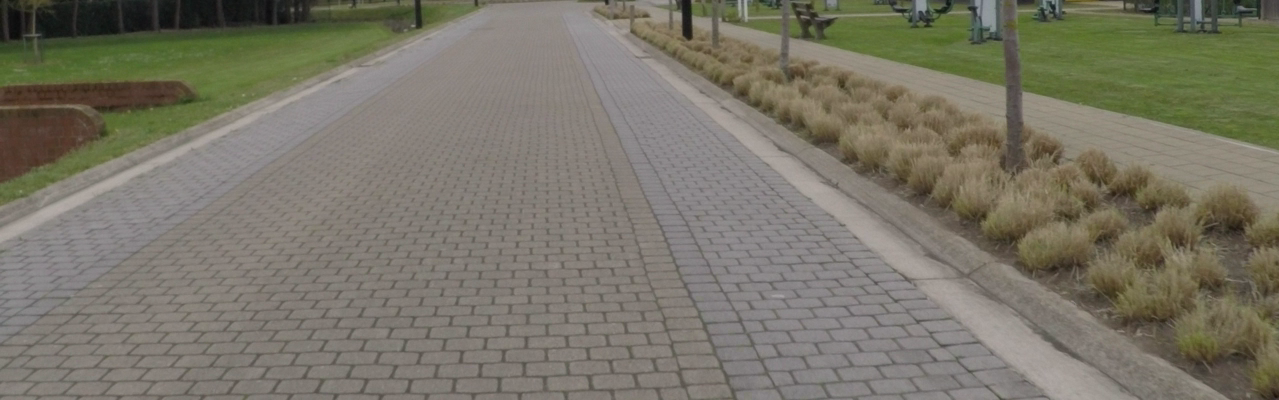
\includegraphics[width=.9\textwidth]{cobbles_in}
  \caption{Original frame\label{cobbles_in}}
\end{subfigure}%
\begin{subfigure}{.5\textwidth}
  \centering
  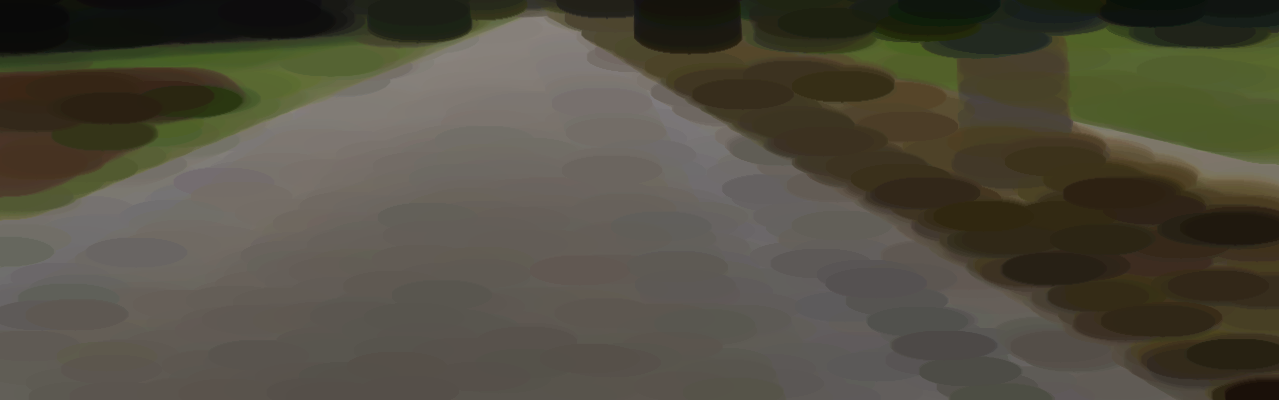
\includegraphics[width=.9\textwidth]{cobbles_erode_out}
  \caption{Eroded cobbled road\label{cobbles_erode_out}}
\end{subfigure}
\caption{Perform eroding to remove the edges on the road.}
\end{figure}


\npar
Eroding is a morphology operator to make the objects on the foreground, which are the brightest, smaller \cite{erode_dilate}. Figure \ref{line_zoom_eroded} shows an example of a thinned white line. When the kernel is large enough, white lines can be filtered out completely. The same technique is used to smooth the surface of cobbled roads. A cobblestone consist of a bright center, surrounded by darker joints. By eroding the cobbled road, the erode function will minimize the center of the cobble, which will cause enlarged joints. With a large kernel, the joints will spread until they overlap. The best results were achieved with an ellipsoidal kernel of 100 x 30 px.

\begin{figure}[ht]
	\begin{minipage}[t]{.45\textwidth}
		\centering
		\begin{subfigure}[t]{.5\textwidth}
		  \centering
		  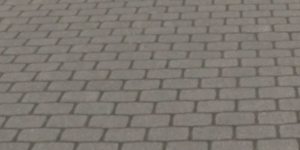
\includegraphics[width=.9\textwidth]{cobbles_zoom_original}
		  \caption{Original frame\label{cobbles_zoom_original}}
		\end{subfigure}%
		\begin{subfigure}[t]{.5\textwidth}
		  \centering
		  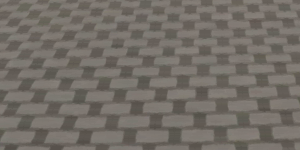
\includegraphics[width=.9\textwidth]{cobbles_zoom_eroded}
		  \caption{Bigger joints after eroding\label{cobbles_zoom_eroded}}
		\end{subfigure}
		\caption{The effect of eroding cobbled roads.}
	\end{minipage}%
	\hspace{0.05\textwidth}
	\begin{minipage}[t]{.45\textwidth}
		\centering
		\begin{subfigure}[t]{.5\textwidth}
		  \centering
		  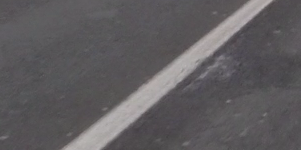
\includegraphics[width=.9\textwidth]{line_zoom_original}
		  \caption{Original frame\label{line_zoom_original}}
		\end{subfigure}%
		\begin{subfigure}[t]{.5\textwidth}
		  \centering
		  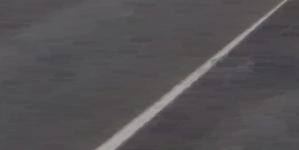
\includegraphics[width=.9\textwidth]{line_zoom_eroded}
		  \caption{Smaller lines after eroding\label{line_zoom_eroded}}
		\end{subfigure}
		\caption{The effect of eroding road markings.}
	\end{minipage}
\end{figure}

\npar
Unfortunately, the erode function will cause the darker objects to expand. The original size of the objects has been modified, as seen in \ref{car_erode_bigger}. This will falsify the eventual edge detection. In this example, the observed car is reported to close. In order to restore the original measures, dilation is executed. This is the opposite morphology operator of eroding. The combination of eroding and dilation is called opening. When dilation is executed with the same kernel size of the erode function, the original size of the dark objects will decrease to their original size, as seen in \ref{car_dilate_smaller}. Note that, after eroding, some details of the shape of the objects are lost. In order to provide a safety margin, the dilate function is executed with a slightly smaller kernel.


\begin{figure}[ht]
\centering
\begin{subfigure}{.5\textwidth}
  \centering
  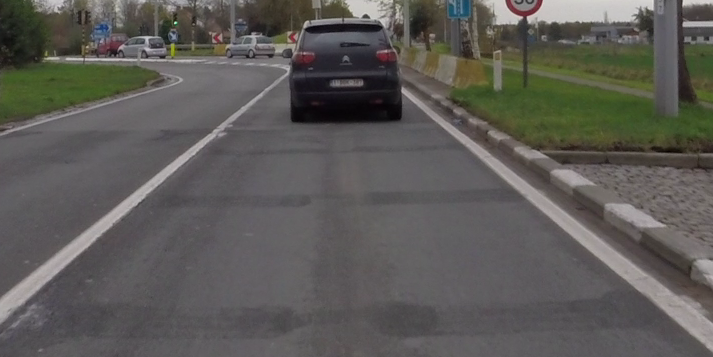
\includegraphics[width=.9\textwidth]{car_original}
  \caption{Original frame\label{car_original}}
\end{subfigure}%
\begin{subfigure}{.5\textwidth}
  \centering
  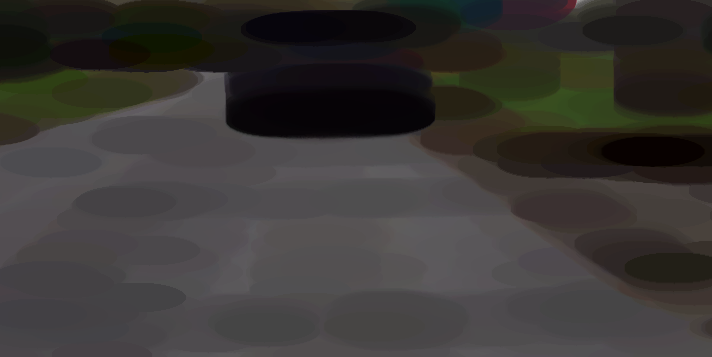
\includegraphics[width=.9\textwidth]{car_erode_bigger}
  \caption{Dark objects are bigger after eroding\label{car_erode_bigger}}
\end{subfigure}
\begin{subfigure}{.5\textwidth}
  \centering
  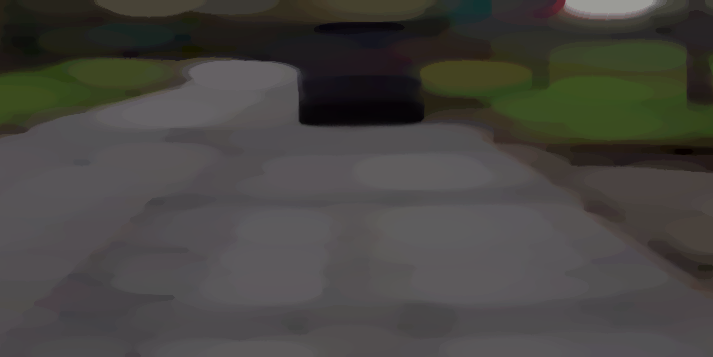
\includegraphics[width=.9\textwidth]{car_dilate_smaller}
  \caption{Restore original sizes with dilation\label{car_dilate_smaller}}
\end{subfigure}
\caption{Perform eroding and dilation to remove details.}
\end{figure}

\subsection{Canny Edge Detection}

To detect the edges of the road, the Canny Edge Detection algorithm is used. Figure \ref{canny_edges} shows an example. 


\begin{figure}[ht]
	\centering
	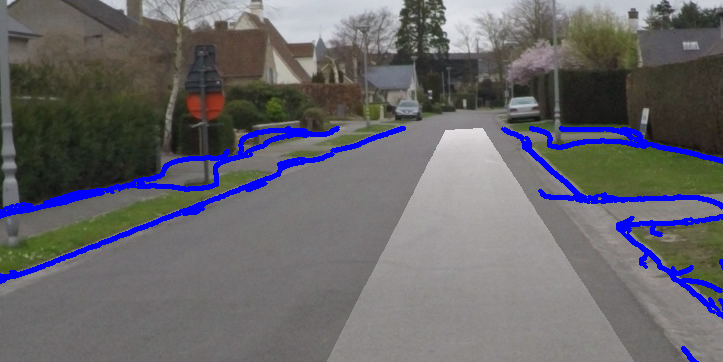
\includegraphics[width=.5\textwidth]{canny_edges}
	\caption{Canny edge detection\label{canny_edges}}
\end{figure}


\npar
This algorithm requires a minimum and a maximum threshold value, which were determined experimentally. 
The best results were achieved with a maximum threshold that is twice the minimum threshold.
The minimum threshold is determined by the required minimum sensitivity. When the algorithm is configured too sensitive, some imperfections on the road will be detected as edges. On the other hand, a certain level of sensitivity is necessary to detect less clear road edges. For example, a transition from road to dirt has a very small distinction of color and brightness, as seen in \ref{transition_road_dirt_eroded}. The minimum threshold should be high enough to detect this transition as edge. 

\begin{figure}[ht]
\centering
\begin{subfigure}{.5\textwidth}
  \centering
  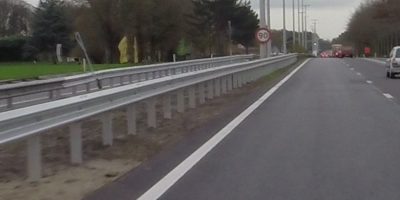
\includegraphics[width=.9\textwidth]{transition_road_dirt_original}
  \caption{Original frame\label{transition_road_dirt_original}}
\end{subfigure}%
\begin{subfigure}{.5\textwidth}
  \centering
  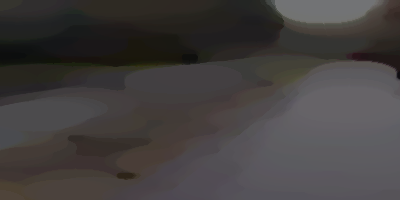
\includegraphics[width=.9\textwidth]{transition_road_dirt_eroded}
  \caption{Eroded road\label{transition_road_dirt_eroded}}
\end{subfigure}
\caption{Unclear transition from road to non-road.}
\end{figure}



\chapter{Conclusie}





% De appendices:
%\appendix

%\input{lc-bijlage-mathsymbols}

% De bibliografie en de index
\backmatter

\bibliography{lc-bibliografie}

\end{document}

